\documentclass[12pt]{article}
\usepackage{times}
\usepackage[utf8]{inputenc}
\usepackage{graphicx}
\usepackage[margin=1in]{geometry}

\setlength{\parindent}{4em}
\setlength{\parskip}{1em}
\renewcommand{\baselinestretch}{1.5}

\author{Bijan Varjavand, Grace Hao, Kevin Necochea}
\title{Error Analysis - How Stiff is Spaghetti}

\begin{document}

\maketitle
\ \\[1in]
\centering
\renewcommand{\baselinestretch}{1.0}
\section{Abstract}
Mastering basic lab techniques, such as error analysis and dimensionless analysis, is a necessity for Materials Science and Engineering students. By thinking critically about the factors which affect the buckling force of spaghetti with different radii and lengths, we apply skills acquired in the classroom to a practical situation. We learned and used specific techniques in order to quantify unique, mechanical properties of different types of spaghetti. The properties of spaghetti in question are the tensile strength and stiffness. The main technique used was measurement of mass, radii, and length in order to determine the buckling force. However, there is an uncertainty associated with every measurement in this experiment. Error analysis is especially important to our calculations because of our lack of precision and, or accuracy in conducting the measurements. 

\clearpage

\raggedright
\linespread{1.6}
\renewcommand{\baselinestretch}{1.5}
\section{Introduction}
Spaghetti is a staple in many diets around the world due to its presence in a variety of pasta dishes. This long, cylindrical pasta is a healthy source of carbohydrates, protein and other vitamins.

Most spaghetti is made from ground grain and water, a mixture which is then dried and packaged for exportation. Distributors must understand the mechanical properties associated with spaghetti in order to limit losses in packaging and processing the material. To accomplish this, they spend time and resources researching how to optimize the mechanical properties of dried spaghetti. Wet and dried spaghetti have very different mechanical properties. Distributors are aware and, thereby, take this into account when generating the final product.

The mechanical properties of a material are those properties that involve a reaction to an applied load. Engineers and manufacturers investigate how materials deform to these loads under certain conditions such as time and temperature. The results obtained might be different depending on the size and shape of tested sample, and even the procedure used to test the properties. Therefore, the ASTM has standard procedures that everyone uses.

In schools, teachers choose spaghetti for science projects because it can be used to learn about how materials bend, a subject in which engineers and materials scientists are very interested. Unlike steel beams, spaghetti is highly affordable and it can help students understand concepts such as tension and compression, concepts which can be applied to any material, not just spaghetti. Spaghetti also exhibits visual response to reasonable levels of stress in classrooms.

In this laboratory experiment, we worked with spaghetti because fairly correct measurements of its mechanical properties can be easily obtained without the need of expensive equipment. We calculated the buckling force associated with three different types of spaghetti at various lengths through compression testing, which can be useful in providing properties such as yield strength, elastic modulus, and ultimate strength.

Also known as Young's modulus, the elastic modulus numerically defines a substance's resistance to being deformed elastically under an applied load. The technical definition is the ratio of stress to strain. Because strain is dimensionless, the units of a material's Young's modulus are pressure units, such as Pa. The elastic modulus of a material lets us predict how much a material sample extends under tension or shortens under compression. From Callister, we found a diagram that explains it well.

\begin{figure}[h]
	\centering
	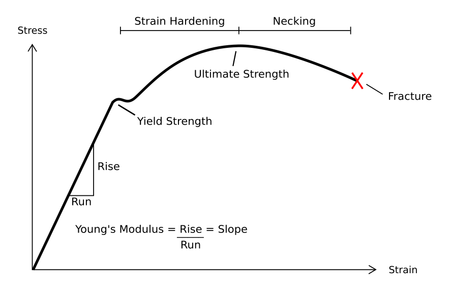
\includegraphics[scale=0.3]{Lab1YM.png}
\end{figure}

Columns under compressive stress can fail in two ways: buckling and crushing. Buckling occurs when a column fails due to bending at a working stress that is less than the ultimate direct stress of the material in question. At this bending point, the force applied can be referred to as the buckling force. An important mechanical property, the Young's modulus is a measure of stiffness of an elastic material, and it can be used to predict elongation or compression.


\section{Procedure}

Our group acquired spaghetti from 3 different boxes - each box contained a different thickness of spaghetti. The thicknesses of the three spaghetti types were measured with calipers, and their lengths were measured with a meter stick. The spaghetti were placed on top of scales, and the weight required to generate a deflection of the spaghetti was measured. The measurements for required weight of noticeable deflection of spaghetti was done repeatedly on the same piece - as 2cm pieces were incrementally cut off. The lengths and weights were recorded, and were used to generate the tables in our appendix.

\section{Results and Discussion}

Three pasta type of ten samples each were tested in order to prove the buckling equation
$$P=E3D4L-264$$
Particularly the exponents of the diameter, m, and the length, n. After testing three different pasta at various lengths, we plotted the log of length vs log of force, which yielded an average slope of -2.1 for n (Fig. 1). This is very close to the expected slope of -2. The log of radius vs log of force plot yielded an average slope of 3.6 for m (Fig. 2), which is somewhat close to the expected slope of 4. We then used our data generated in lab and the buckling equation to solve for the Young's Modulus $$E=P3DmLn64$$. We averaged the Young's modulus associated with the different lengths and types of pasta to get a Young's Modulus of $2.32 GPa \pm 0.22 GPa$. The Young's Modulus of spaghetti is 5.0 GPa (expected). Our results differed greatly, with a factor of 2, compared to the literature value of spaghetti.

Although our Young's Modulus was very precise, it was highly inaccurate because of how it deviates from the literature values. This is due to inaccuracy of which we were conducting the experiment to measure the buckling force. We used calipers to measure diameter of the different types of spaghetti, which has an uncertainty of 0.5mm, making this measurement highly accurate. However, the scale had an uncertainty of 0.001kg associated with it, which is similar to the weight of the heaviest pasta strand we measured (0.0012kg).The scale's uncertainty was a major contributor to the error that happened within this experiment as well as human error.  To find the n value of the buckling of spaghetti, we measured various lengths using a ruler that had an uncertainty of 0.05cm. The main error in our measurements was from the visual detection of noticeable deflection in spaghetti. A person cannot judge by eye the same exact bending in the spaghetti and record the weight that is exerted associated with the bending. We also had a different person measure the buckling force for each type of spaghetti. Not only is each person’s judgement of the buckling force extremely different, but we also cut the spaghetti differently, with two people using a knife, while another measured the 2cm increment and broke spaghetti and the marked spot. We didn't expect our values to be close the literature value of spaghetti because before starting the experiment, we noted how large human error and the scale inaccuracy would be in this experiment. The preciseness of our measurement shows that the experiment was minimized as our error was relatively small, even though our value differed greatly compared to the literature value.

\section{Error Analysis}

Our buckling load equation is
$$P = \frac{E\pi ^3D^3}{4L^2}$$
$$E = \frac{4PL^2}{\pi ^3D^4}$$

We can confirm the powers by plotting the data on log scales.

\begin{figure}[h]
	\begin{minipage}{0.5\textwidth}
		\centering
		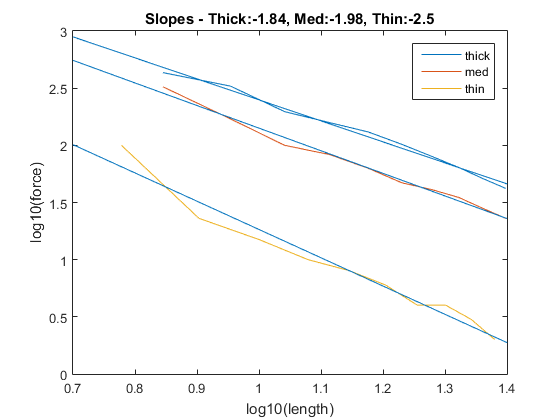
\includegraphics[scale=0.3]{Lab1f1.png}
		\caption{Average for slopes = -2.1}
	\end{minipage}%
	\begin{minipage}{0.5\textwidth}
		\centering
		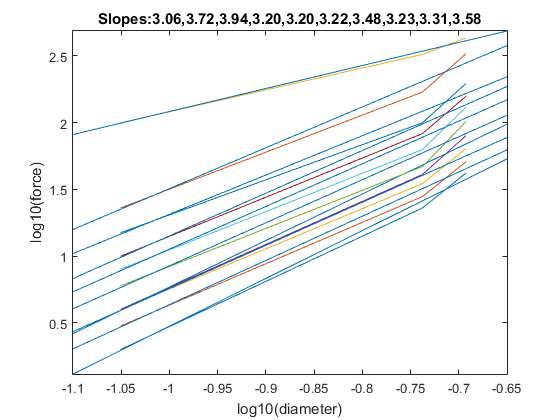
\includegraphics[scale=0.3]{Lab1f3.png}
		\caption{Average for slopes = 3.6}
	\end{minipage}
\end{figure}

Solving for E using our equation, we get 30 values from all our data points. Averaging the E values, we get 2.32 GPa.

The ruler we used had an error of $\pm$ 0.5mm, and the scale had an error of $\pm$ 1g. Converting error from the scale into Newtons, it becomes $\pm$ 0.0098N.

Error propagation given by
$$\frac{\delta E}{E} = \frac{4}{\pi ^3}\sqrt{(\frac{4\delta L}{L})^2 + (\frac{2\delta D}{D})^2 + (\frac{\delta P}{P})^2}$$

$$\frac{\delta E}{E} = \frac{4}{\pi ^3}\sqrt{(\frac{4(0.05cm)}{L})^2 + (\frac{2(0.05cm)}{D})^2 + (\frac{(0.001kg)}{P})^2}$$

I found $\frac{\delta e}{E}$ values for all 30 data points, then averaged all of them to get $\frac{\delta E}{E}$ = 0.0967. Multiplying by the value for E we found, we get $\delta E$ = 224 MPa. This results in $$2.32GPa \pm 0.22GPa$$

\section{Appendix}
\centering
\begin{tabular}{|| c | c | c | c ||}
 \hline
 Thick &\ &\ &\ \\
 \hline
 Length(cm) & Mass(g) & Force(N) & Diameter(cm) \\
 \hline
 \hline
 25 & 42 & 412.02 & 0.203 \\
 23 & 51 & 500.31 &\ \\
 21 & 64 & 627.84 &\ \\
 19 & 80 & 784.80 &\ \\
 17 & 102 & 1000.62 &\ \\
 15 & 131 & 1285.11 &\ \\
 13 & 158 & 1549.98 &\ \\
 11 & 197 & 1932.57 &\ \\
 9 & 329 & 3227.49 &\ \\
 7 & 432 & 4237.92 &\ \\
 \hline
\end{tabular}\\\ \\\ \\\ 

\centering
\begin{tabular}{|| c | c | c | c ||}
 \hline
 Medium &\ &\ &\ \\
 \hline
 Length(cm) & Mass(g) & Force(N) & Diameter(cm) \\
 \hline
 \hline
 25 & 23 & 225.63 & 0.183\\
 23 & 28 & 274.68 &\ \\
 21 & 35 & 343.35 &\ \\
 19 & 41 & 402.21 &\ \\
 17 & 47 & 461.07 &\ \\
 15 & 63 & 618.03 &\ \\
 13 & 83 & 814.23 &\ \\
 11 & 100 & 981.00 &\ \\
 9 & 170 & 1667.70 &\ \\
 7 & 325 & 3188.25 &\ \\
 \hline
\end{tabular}\\\ \\\ \\\ 

\centering
\begin{tabular}{|| c | c | c | c ||}
 \hline
 Thin &\ &\ &\ \\
 \hline
 Length(cm) & Mass(g) & Force(N) & Diameter(cm) \\
 \hline
 \hline
 24 & 2 & 19.62 & 0.089\\
 22 & 3 & 29.43 &\ \\
 20 & 4 & 39.24 &\ \\
 18 & 4 & 39.24 &\ \\
 16 & 6 & 58.86 &\ \\
 14 & 8 & 78.48 &\ \\
 12 & 10 & 98.10 &\ \\
 10 & 15 & 147.15 &\ \\
 8 & 23 & 225.63 &\ \\
 6 & 100 & 981.00 &\ \\
 \hline
\end{tabular}

\end{document}